% Chapter 5

\chapter{Bilan du stage} % 5th chapter title

\label{Chapter5} % For referencing the chapter elsewhere, use \ref{Chapter5} 

%----------------------------------------------------------------------------------------

\section{Ressources utilisées}

Les ressources utilisee durant le stage varient en nature et en fonction.

\subsection{Ecriture du Code}
\begin{itemize}
 \item VSCode: Pour l'edition du (principalemtn C++) grace a ses fonction. L'extension majeure ici est CMake.
 \item Google Colab: Facilitation de l'apprentissage sous Keras grace a ses GPU. Les libraries majeures ici sont Numpy, pandans, et Keras.
 \item Jupyter: Pour les taches en Python ne necessitant pas trop de resource (visualisation, sauvegarde en format PQT). Les librairies majeures utilisees ici sont Numpy, Pandas et Matplotlib.
 \item Kile: Pour l'ecritude du rapport en Latex
 \item Draw.io: Pour les illustrations 
\end{itemize}


\subsection{Communication}
Les communications se sont effectuees principalemtn par messagerie electronique. j'ai aussi eu l'occasion de communiquer avec les proffeseurs en presentiel a 3 reprise.

%----------------------------------------------------------------------------------------

\section{Journal de bord}
\label{sec:Journal}

\subsection{Semaine 1 et 2}
\begin{itemize}
 \item 15 juin: Reunion de debut de Stage par Google Meet
 \item 16 juin: Demande aux professeurs de verifier un example de simulation 1D, avant de me lancer la generation des donnnees
 \item 17 juin: Remarque du problem d'apparition du crenau sur l'energie 
 \item 18 juin: Redaction d'un nouveau schema par M. Franck (pour l'etape 1) qui devrait conserver l'equilibre
 \item 22 juin: Detection de la source du probleme du crenau sur E, et redefinition des termes. 
 \item 23 juin: Confirmation de l'exactitude des simulations 1D et debut de la generation des donnes avec 500 mailles.
\item 25 juin: Demande d'aide a M. Vigon pour la configuration de la fonction d'activation de la couche de sortie
\end{itemize}


\subsection{Semaine 3 et 4}

\begin{itemize}
 \item 3 juillet: Rencontre avec M. Navoret pour discuter des avancements. Prise de connaissance de d'une des raisons potentielles du probleme de mauvaise prediction de la position du crenau sur la densite en 1D. Proposition de plusieurs solutions par M. Navoret, entre autre de partir d'un signal stationanire sinnusoidal et d'introduire l'onde a un temps t*>0.
 \item 6 juillet: Nouvelles simualtions effectues en vue d'observer la difference entre les effets de deux densites differentes. Continuation vers des nouvelles simualtiosn avec 300 mailles.
 \item 8 juillet: decroissance du taux d'apprentissage a la suggestion de M. Franck mais non amelioration des resultats d'apprentissage.
 \item 9 juillet: Passage aux reseaux convolutif grace a M. Vigon
 \item 11 juillet: Plot du debut des oscillation, des maximum, des minimum a la demande de M. Vigon, afin de mieux observer les effet de deux crenaux de densite diferents. 
\end{itemize}

\subsection{Semaine 5 et 6}

\begin{itemize}
 \item 13 juillet: Rencontre avec M. Navoret et M. Franck a la fac. Denvant la persistance du probleme de non detection de la position du crenau, l'implementation du probleme en 2D semble etre la solution approprie.
 \item 14 juillet reformulation 2D du schema de splitting et adaptation du code 1D en 2D
 \item 19 juillet: fin du codage 2D  er presentation des resultats
 \item 25 juillet: ajustemetn de la gamme de couleurs pour les visualisations et passage a la generation des donnes sur 90x90 mailles.
\end{itemize}

\subsection{Semaine 7, 8, et 9}
\begin{itemize}
 \item 5 aout: Rencontre avec M. Franck a la fac. Proposition de solutions pour la non dectection de la position du crenau en 2D par resolution d'un systeme proche de l'eq de la chaleur, apres affichage par ligne de niveau. La possibilite d'adopter un obstacle s'etendant sur toute la verticale est envidagee. Prise de connaissance des delains pour la redaction du rapport.
 \item 6 aout: Redaction et envoi du plan du rapport de stage. 
 \item 7 sout: Proposition de reduction drasque de resolution spatiale par M. Vigonm, et proposition de nouvelles idees par M. Vigon, entre autre la consideration d'un obstacle considerableme plus opaque.
 \item 8 sout: Nouvel apprentissage avec des simplification majeures qui fonctionnne. Melioration des resultats et continuation du rapport.
 \item 15 aout: Soumission du premier brouillon du rapport
\end{itemize}
%----------------------------------------------------------------------------------------

\section{Difficultés rencontrées et solutions apportées}

Un resume du deroulement du stage est presente a la figure \ref{fig:MilestonesRoadmap}. Les points tounant les plus marquants du stage y sont representes. On peut aussi y voire les diffultes majeures auquelles j'ai ete confronte.

\begin{figure}[H] 
\centering
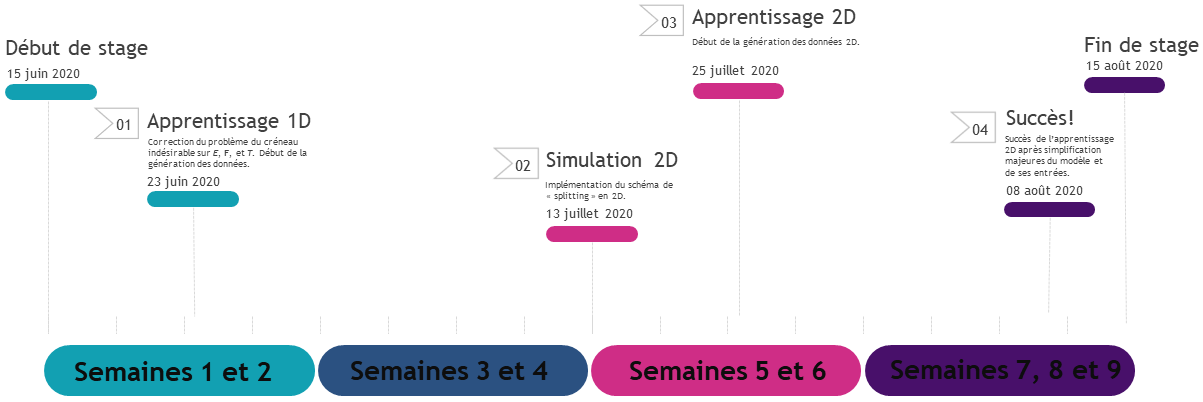
\includegraphics[width=.8\linewidth]{MilestonesRoadmap} 
\decoRule
\caption[MilestonesRoadmap]{Resumes des etapes marquantes du stage. Les details du deroulement peuvent etre obtenues dans la section \ref{sec:Journal}.}
\label{fig:MilestonesRoadmap}
\end{figure}

\subsection{Apparition d'un crenau sur E, F, et T}
Au commencement du stage, le code de calcul 1D n'etait pas au point. En effet, des qu'on placait un crenau sur la densite, un crenau correpondant se formait puis se propageait sur les signaux E, F, et T. Le probleme a ete resolu par rajout d'un terme au niveau de la deuxieme equation du schema de splitting.

\subsection{Detection de la position du crenau}
La detection de la position du saut de densite a ete un probleme majeure durant le stage. A la fin stage, aucune solution (si elle existe) n'a ete trouvee pour le probleme inverse en 1D. 
Cependant en 2D le probleme a ete resolu essentiellment par augmentation du nombre d'epoques et dimunution du taux d'appretissagee a 1e-5. Il est bien connu que les problemes de machine peuvent diverger si le taux d'apprentissage est trop eleve. Quand au nombre d'eqpoques, je n'en faisait pas suffisament pour voir le modele converger. Une solution bien plus rapide aurait ete d'automatiser la recherche des hyper-parametres, chose que je n'ai apprise qu'a la fin du stage.

Pour revenir a l'apprentissage en 1D, il est important de mentionner quelques pistes d'etude qui, combinee, auraient pu ameliorer les resultats ():
\begin{itemize}
    \item deux apprentissage different: en creant un modele separes pour l'apprentissage de la postion  et de la hauteur
    \item elimination des mauvais labels: on pourrait supprimer de l'appretissage tous les examples qui ont un label trop proche du bord du domaine (par exemple compris entre 0.2 et 0.8 comme en 2D).
\end{itemize}

Cela dit, la solution touvee en 2D est loin d'etre optimale; elle souffre de deux problemes majeures:
\begin{itemize}
 \item pas de generalisation: le modele finalement retenu ne comporte pas de couche de maxpooling
 \item modle trop lourd: le nombre de parametres est tres eleve du a la taille des entree (168, 28, 48) ce qui conduit a un espace memoire tres important au moment de la sauvegarde des poids.
\end{itemize}

Toutes ces quatres pistes d'amelioration n'ont pas ete implemntee pour cause de temps. La gestion de temps a ete un vrai probleme lors du stage.

\subsection{Gestion du temps}
La gestion du temps durant le stage n'a aps ete facile. Au moment d'imimpplementer le schema en 2D (ce qui n'etait pas initialement prevu), j'ai longement hesiter sur l'option la plus rapide. J'ai pu compter sur les conseils de M. Navoret pour surmonter cet obstacle. 

Aussi, je me suis rendu compte des delais bien en retard, j'ai du me debrouiller pour ameliorer les resultat et terminer l'apprentissage. Cela dit, je n'ai pas reussi a faire une partie essentielle qui consiste a verfier comment un modele un modele avec MaxPooling se generalise mieux qu'un modele sans.

%----------------------------------------------------------------------------------------

\section{Les apports du stage}

Ce stage a ete enrichissant pour moi sur plusieurs front:

\subsection{Experience en developpement}
J'ai gagne de l'experience en development C++ et Python, tout en me developant un portfolio. J'ai beaocup apris sur l'API de Pandas, Matplotlib, et plus important encore, celle de Keras. J'ai a present une large base de donnes de code reutilisable pour d'autres taches.

\subsection{Equations aux derivee aprtielles}
J'ai pu observer directemnt quelques astuces utilisees par mes maitres de stages pour verfier la validite de la modelisatopm d'une EDP. Pour l'equation du transfer radiatif, j'ai compris la necessite de partir d'un etat d'equilibre radiatif.

\subsection{Reseau de neurones}
Ce stage m'a permis de percevori la puissance des reseaux de neurones. J'ai appris a quel point le taux d'apprentissage est important. Comme mentionne dans le livre de reference Deep learning \textit{The learning rate is perhaps the most important hyperparameter. If you have time to tune only one hyperparameter, tune the learning rate} \parencite[417]{Reference5}. 

J'en ressort aussi avec quelques question concernant le batch size. Lors de l'apprentissage, il a fallu entrainer le modele en utlisant la methode d'augmentation du batch size pour obtenir les premiers "bons" resultats. Cette methode referencee ici (LiEN RETROUVABLE DANS LES MAIL) montre que beacoupd de questions restent a resoudre dans le domaine du deep learning.

\subsection{Experience de recherche}
En tant que premiere experience dans un environnement de recherche tel que l'UFR, j'ai pu me familirser avec le milieu. J'ai notament apris que les resultats ne doivent pas toujours etre ceux auxquels on s'attends, du moment que l'on a une explication de l'echer.

%----------------------------------------------------------------------------------------
